\documentclass[french,]{compterendu}
\usepackage{lmodern}
\usepackage{amssymb,amsmath}
\usepackage{ifxetex,ifluatex}
\usepackage{fixltx2e} % provides \textsubscript
\ifnum 0\ifxetex 1\fi\ifluatex 1\fi=0 % if pdftex
  \usepackage[T1]{fontenc}
  \usepackage[utf8]{inputenc}
\else % if luatex or xelatex
  \ifxetex
    \usepackage{mathspec}
  \else
    \usepackage{fontspec}
  \fi
  \defaultfontfeatures{Ligatures=TeX,Scale=MatchLowercase}
\fi
% use upquote if available, for straight quotes in verbatim environments
\IfFileExists{upquote.sty}{\usepackage{upquote}}{}
% use microtype if available
\IfFileExists{microtype.sty}{%
\usepackage{microtype}
\UseMicrotypeSet[protrusion]{basicmath} % disable protrusion for tt fonts
}{}
\usepackage[left=2cm,right=2cm,top=2.5cm,bottom=2.5cm]{geometry}
\usepackage{hyperref}
\hypersetup{unicode=true,
            pdftitle={Un titre évocateur et relativement court pour le compte-rendu},
            pdfauthor={Premier AUTEUR},
            pdfkeywords={Schtroumpf; Marsupilami; Pokemon},
            pdfborder={0 0 0},
            breaklinks=true}
\urlstyle{same}  % don't use monospace font for urls
\ifnum 0\ifxetex 1\fi\ifluatex 1\fi=0 % if pdftex
  \usepackage[shorthands=off,main=french]{babel}
\else
  \usepackage{csquotes}
  \usepackage{polyglossia}
  \setmainlanguage[]{}
\fi
\usepackage[style=alphabetic]{biblatex}

\addbibresource{biblio-cr-urca.bib}
% Adding environment CSLReferences for compatibility with pandoc >= 2.8
% BEGIN

\newlength{\cslhangindent}
\setlength{\cslhangindent}{1.5em}
\newlength{\csllabelwidth}
\setlength{\csllabelwidth}{3em}
\newenvironment{CSLReferences}[2] % #1 hanging-ident, #2 entry spacing
 {% don't indent paragraphs
  \setlength{\parindent}{0pt}
  % turn on hanging indent if param 1 is 1
  \ifodd #1 \everypar{\setlength{\hangindent}{\cslhangindent}}\ignorespaces\fi
  % set entry spacing
  \ifnum #2 > 0
  \setlength{\parskip}{#2\baselineskip}
  \fi
 }%
 {}
\usepackage{calc} % for \widthof, \maxof
\newcommand{\CSLBlock}[1]{#1\hfill\break}
\newcommand{\CSLLeftMargin}[1]{\parbox[t]{\maxof{\widthof{#1}}{\csllabelwidth}}{#1}}
\newcommand{\CSLRightInline}[1]{\parbox[t]{\linewidth}{#1}}
\newcommand{\CSLIndent}[1]{\hspace{\cslhangindent}#1}

% END
\usepackage{color}
\usepackage{fancyvrb}
\newcommand{\VerbBar}{|}
\newcommand{\VERB}{\Verb[commandchars=\\\{\}]}
\DefineVerbatimEnvironment{Highlighting}{Verbatim}{commandchars=\\\{\}}
% Add ',fontsize=\small' for more characters per line
\usepackage{framed}
\definecolor{shadecolor}{RGB}{248,248,248}
\newenvironment{Shaded}{\begin{snugshade}}{\end{snugshade}}
\newcommand{\AlertTok}[1]{\textcolor[rgb]{0.94,0.16,0.16}{#1}}
\newcommand{\AnnotationTok}[1]{\textcolor[rgb]{0.56,0.35,0.01}{\textbf{\textit{#1}}}}
\newcommand{\AttributeTok}[1]{\textcolor[rgb]{0.13,0.29,0.53}{#1}}
\newcommand{\BaseNTok}[1]{\textcolor[rgb]{0.00,0.00,0.81}{#1}}
\newcommand{\BuiltInTok}[1]{#1}
\newcommand{\CharTok}[1]{\textcolor[rgb]{0.31,0.60,0.02}{#1}}
\newcommand{\CommentTok}[1]{\textcolor[rgb]{0.56,0.35,0.01}{\textit{#1}}}
\newcommand{\CommentVarTok}[1]{\textcolor[rgb]{0.56,0.35,0.01}{\textbf{\textit{#1}}}}
\newcommand{\ConstantTok}[1]{\textcolor[rgb]{0.56,0.35,0.01}{#1}}
\newcommand{\ControlFlowTok}[1]{\textcolor[rgb]{0.13,0.29,0.53}{\textbf{#1}}}
\newcommand{\DataTypeTok}[1]{\textcolor[rgb]{0.13,0.29,0.53}{#1}}
\newcommand{\DecValTok}[1]{\textcolor[rgb]{0.00,0.00,0.81}{#1}}
\newcommand{\DocumentationTok}[1]{\textcolor[rgb]{0.56,0.35,0.01}{\textbf{\textit{#1}}}}
\newcommand{\ErrorTok}[1]{\textcolor[rgb]{0.64,0.00,0.00}{\textbf{#1}}}
\newcommand{\ExtensionTok}[1]{#1}
\newcommand{\FloatTok}[1]{\textcolor[rgb]{0.00,0.00,0.81}{#1}}
\newcommand{\FunctionTok}[1]{\textcolor[rgb]{0.13,0.29,0.53}{\textbf{#1}}}
\newcommand{\ImportTok}[1]{#1}
\newcommand{\InformationTok}[1]{\textcolor[rgb]{0.56,0.35,0.01}{\textbf{\textit{#1}}}}
\newcommand{\KeywordTok}[1]{\textcolor[rgb]{0.13,0.29,0.53}{\textbf{#1}}}
\newcommand{\NormalTok}[1]{#1}
\newcommand{\OperatorTok}[1]{\textcolor[rgb]{0.81,0.36,0.00}{\textbf{#1}}}
\newcommand{\OtherTok}[1]{\textcolor[rgb]{0.56,0.35,0.01}{#1}}
\newcommand{\PreprocessorTok}[1]{\textcolor[rgb]{0.56,0.35,0.01}{\textit{#1}}}
\newcommand{\RegionMarkerTok}[1]{#1}
\newcommand{\SpecialCharTok}[1]{\textcolor[rgb]{0.81,0.36,0.00}{\textbf{#1}}}
\newcommand{\SpecialStringTok}[1]{\textcolor[rgb]{0.31,0.60,0.02}{#1}}
\newcommand{\StringTok}[1]{\textcolor[rgb]{0.31,0.60,0.02}{#1}}
\newcommand{\VariableTok}[1]{\textcolor[rgb]{0.00,0.00,0.00}{#1}}
\newcommand{\VerbatimStringTok}[1]{\textcolor[rgb]{0.31,0.60,0.02}{#1}}
\newcommand{\WarningTok}[1]{\textcolor[rgb]{0.56,0.35,0.01}{\textbf{\textit{#1}}}}
\usepackage{longtable,booktabs}
\usepackage{graphicx,grffile}
\makeatletter
\def\maxwidth{\ifdim\Gin@nat@width>\linewidth\linewidth\else\Gin@nat@width\fi}
\def\maxheight{\ifdim\Gin@nat@height>\textheight\textheight\else\Gin@nat@height\fi}
\makeatother
% Scale images if necessary, so that they will not overflow the page
% margins by default, and it is still possible to overwrite the defaults
% using explicit options in \includegraphics[width, height, ...]{}
\setkeys{Gin}{width=\maxwidth,height=\maxheight,keepaspectratio}
\IfFileExists{parskip.sty}{%
\usepackage{parskip}
}{% else
\setlength{\parindent}{0pt}
\setlength{\parskip}{6pt plus 2pt minus 1pt}
}
\setlength{\emergencystretch}{3em}  % prevent overfull lines
\providecommand{\tightlist}{%
  \setlength{\itemsep}{0pt}\setlength{\parskip}{0pt}}
\setcounter{secnumdepth}{5}
% Redefines (sub)paragraphs to behave more like sections
\ifx\paragraph\undefined\else
\let\oldparagraph\paragraph
\renewcommand{\paragraph}[1]{\oldparagraph{#1}\mbox{}}
\fi
\ifx\subparagraph\undefined\else
\let\oldsubparagraph\subparagraph
\renewcommand{\subparagraph}[1]{\oldsubparagraph{#1}\mbox{}}
\fi

%%% Use protect on footnotes to avoid problems with footnotes in titles
\let\rmarkdownfootnote\footnote%
\def\footnote{\protect\rmarkdownfootnote}



%Mise en page
%\usepackage[left=2cm,right=2cm,top=2cm,bottom=2.5cm]{geometry}
%\usepackage{lastpage} %Pour numérotaion des pages
\usepackage{eso-pic} %pour l'image de fond de la page de garde
\usepackage{enumitem} %Pour personnaliser les listes à puces
\usepackage{fancyhdr}
\usepackage{xcolor}
\usepackage[T1]{fontenc}
\usepackage{amsthm}
%\usepackage{thmtools}

\usepackage[figure,table]{totalcount} % Pour avoir les nombres de figures, tables et théoremes
\usepackage{totcount} % Pour compter le nombre de références

%Gestion des tableaux
\usepackage{multirow}
\usepackage{float}
\floatplacement{table}{H}
\floatplacement{figure}{ht!}

%Divers
\usepackage{ifthen} %Gestion des instructions conditionnelles

% % Gestion de la bibliographie
% \usepackage[sorting=none, backend=biber]{biblatex}
% \addbibresource{biblio_cr-urca.bib}

\widowpenalty=10000
\clubpenalty=10000

%%%%%%%%%%%%%%%%%%%%%%%%%%%
%% Defining new counters %%
%%%%%%%%%%%%%%%%%%%%%%%%%%%

%% Compteur des références
\newtotcounter{citenum} %From the package documentation
\def\oldbibitem{} \let\oldbibitem=\bibitem
\def\bibitem{\stepcounter{citenum}\oldbibitem}




\regtotcounter{figure}
\regtotcounter{table}
\regtotcounter{theorem}


%%%%%%%%%%%%%%%%%%%%%%%%%%%%%%%%%%%%%%%%%%%%%%%
%% Configuration des messages de type badbox %%
%%%%%%%%%%%%%%%%%%%%%%%%%%%%%%%%%%%%%%%%%%%%%%%

\widowpenalty=10000
\clubpenalty=10000


%%%%%%%%%%%%%%%%%%%%%%%%%%%%
%% Theorem environemments %%
%%%%%%%%%%%%%%%%%%%%%%%%%%%%


\theoremstyle{urcastyle}
\newtheorem{theorem}{Théorème}
\newtheorem{lemma}{Lemme}
\newtheorem{corollary}{Corollaire}
\newtheorem{proposition}{Proposition}
\newtheorem{definition}{Définition}
\newtheorem{example}{Exemple}

\theoremstyle{remark}
%\newtheorem*{proof}{Démonstration}


%%%%%%%%%%%%%%%%%%%%%%%%%%%%%%%%%%%%%%%%%%%%
%% Désignation des variables de la classe %%
%%%%%%%%%%%%%%%%%%%%%%%%%%%%%%%%%%%%%%%%%%%%

% Processing title
  \newcommand{\titlehead}{Un titre évocateur et relativement court pour le compte-rendu}
  \title{Un titre évocateur et relativement court pour le compte-rendu}
    % Processing authors
  \newcounter{nbaut}
  \setcounter{nbaut}{1} % Nombre d'auteurs
  \author{Premier AUTEUR}
      \date{10 décembre 2024}

 \resume{Un paragraphe présentant de façon synthétique le contenu du compte-rendu. \newline Il est possible de faire des retours à la ligne. Et d'insérer des commandes \LaTeX à condition de doubler les anti-slashs. On peut aussi y glisser du code R avec la syntaxe de R Markdown ; ainsi, R nous apprend que \(3\times4\) valent 12.}
 \keywords{Schtroumpf, Marsupilami, Pokemon.}

 \gitrepo{\url{https://github.com/pregnault/urcadown}}
 \database{\url{https://data.gouv.fr}}


 \coefficient{40 \%}

\usepackage{booktabs}
\usepackage{longtable}
\usepackage{array}
\usepackage{multirow}
\usepackage{wrapfig}
\usepackage{float}
\usepackage{colortbl}
\usepackage{pdflscape}
\usepackage{tabu}
\usepackage{threeparttable}
\usepackage{threeparttablex}
\usepackage[normalem]{ulem}
\usepackage{makecell}
\usepackage{xcolor}

  \email{\href{mailto:premier.auteur@univ-reims.fr}{\nolinkurl{premier.auteur@univ-reims.fr}}}
%\email{\href{mailto:premier.auteur@univ-reims.fr}{\nolinkurl{premier.auteur@univ-reims.fr}}}
\logouniv{logo_URCA.pdf}
\logoufr{logoSEN.pdf}
\date{10 décembre 2024}
\diplome{Licence Mathématiques Appliquées, 3\up{ème} année}
\anac{2021-2022}
\module{MA0606}
\enseig{Philippe Regnault}
\evaluation{Compte-rendu d'analyse}

%% Passage des compteurs à la classe pour maketitle.
\totfig{\total{figure}}
\tottab{\total{table}}
\totref{\total{citenum}}
\tottheo{\total{theorem}}

%%%%%%%%%%%%%%%%%%%
%% Mise en forme %%
%%%%%%%%%%%%%%%%%%%


%Formatage en-têtes et pieds de pages
\pagestyle{fancy}
\fancyhead[L]{\small \titlehead}
%\fancyhead[C]{\small \textcolor{urcabrown}{\titlehead}}
\fancyhead[R]{}
\fancyfoot[l]{\small \ifnum \value{nbaut}=1 {Premier AUTEUR} \else {Premier AUTEUR \textit{et al.}}\fi}
\fancyfoot[C]{\small \it \theeval \ \themodule \ -- \theanac}
\fancyfoot[R]{\small \thepage\ / \pageref{LastPage}}
% \renewcommand{\headrule}{\hbox to\headwidth{%
%     \color{urcabrown}\leaders\hrule height \headrulewidth\hfill}}
% \renewcommand{\footrule}{\hbox to\headwidth{%
%     \color{urcabrown}\leaders\hrule height \headrulewidth\hfill}}
\renewcommand{\headrulewidth}{0.5pt}
\renewcommand{\footrulewidth}{0.5pt}

\renewcommand{\headrulewidth}{0.5pt}
\renewcommand{\footrulewidth}{0.5pt}

\fancypagestyle{plain}{%
\fancyhf{} % clear all header and footer fields
\fancyfoot[C]{\small \thepage\ / \pageref{LastPage}} % except the center
\renewcommand{\headrulewidth}{0pt}
\renewcommand{\footrulewidth}{0pt}}

\AtEndDocument{\thispagestyle{plain}}
% Pandoc header
  \usepackage{booktabs}
  \usepackage{longtable}
  \usepackage{array}
  \usepackage{multirow}
  \usepackage{wrapfig}
  \usepackage{float}
  \usepackage{colortbl}
  \usepackage{pdflscape}
  \usepackage{tabu}
  \usepackage{threeparttable}
  \usepackage{threeparttablex}
  \usepackage[normalem]{ulem}
  \usepackage{makecell}
  \usepackage{xcolor}


%%%%%%%%%%%%%%%%%%%%%%%
%% Début du document %%
%%%%%%%%%%%%%%%%%%%%%%%

\begin{document}

\AddToShipoutPictureBG*{
\includegraphics[width=\paperwidth,height=\paperheight]{fond_a4_sen_3.pdf}}

% \theoremstyle{urca}
\newtheorem{lemme}{Lemme}[section]
\newtheorem{theoreme}{Théorème}[section]
% \newtheorem{proposition}{Proposition}[section]
% \newtheorem{definition}{Définition}[section]
\newtheorem{corollaire}{Corollaire}[section]
\newtheorem{propriete}{Propriété}[section]
\newtheorem{proprietes}{Propriétés}[section]



\maketitle

% \pagebreak
% 
% % \begin{abstract}
% Un paragraphe présentant de façon synthétique le contenu du compte-rendu. \newline Il est possible de faire des retours à la ligne. Et d'insérer des commandes \LaTeX à condition de doubler les anti-slashs. On peut aussi y glisser du code R avec la syntaxe de R Markdown ; ainsi, R nous apprend que \(3\times4\) valent 12.
% \end{abstract}
% 

% \vspace{1cm}
% 
% Test afficher le nombre de citations : \total{citenum}


  {
  \hypersetup{linkcolor=black}
  \setcounter{tocdepth}{2}
  \tableofcontents
  }

\pagebreak
\normalsize



\section{Première partie}\label{premiuxe8re-partie}

\subsection{Avec une première sous-partie}\label{avec-une-premiuxe8re-sous-partie}

Le corps du document est rédigé selon la syntaxe de \emph{Markdown}. On peut mettre des expressions en \emph{italique} ou en \textbf{gras}, des blocs de code en ligne (non évalués) comme celui-ci \texttt{sample(1:49,\ 6)}, insérer des commentaires de base de page\footnote{Ceci est un commentaire de bas de page.}, des liens hypertexte comme \href{http://univ-reims.fr}{celui-là}, des expressions mathématiques exprimées selon la syntaxe de \LaTeX, du genre \(\cos(\theta) ^2 + \sin(\theta)^2 = 1\), voire les centrer comme ceci :
\[(a+b)^n = \sum_{k=0}^n {n \choose k} a^k b^{n-k}, \quad a,b \in \mathbb{C}, \quad n \in \mathbb{N}.\]

\subsection{Puis une seconde}\label{puis-une-seconde}

On peut également insérer des blocs de code R dont le rendu est paramétrable. Par exemple, le bloc suivant est affiché sans être évalué

\begin{Shaded}
\begin{Highlighting}[]
\FunctionTok{sample}\NormalTok{(}\DecValTok{1}\SpecialCharTok{:}\DecValTok{49}\NormalTok{, }\DecValTok{6}\NormalTok{)}
\end{Highlighting}
\end{Shaded}

tandis que la sortie suivante est affichée sans que le code exécuté n'apparaisse :

\begin{verbatim}
## 
##  Pearson's Chi-squared test
## 
## data:  un_tableau
## X-squared = 2.8687, df = 6, p-value = 0.8251
\end{verbatim}

On peut également insérer du code R en ligne, qui sera remplacé par le résultat de son évaluation dans le document généré, par exemple, le résultat de \(3 \times 4\) vaut 12.

\section{Deuxième partie}\label{deuxiuxe8me-partie}

Le template \texttt{cr-urca} utilise le package \textbf{bookdown} \autocite{pkgbookdown} apportant quelques fonctionnalités supplémentaires, dont la gestion des références croisées et des citations. La Figure \ref{fig:dotplotex} donne un exemple de graphique accompagné de sa légende.






\begin{Shaded}
\begin{Highlighting}[]
\FunctionTok{library}\NormalTok{(}\StringTok{"ggplot2"}\NormalTok{)}
\FunctionTok{ggplot}\NormalTok{(}\AttributeTok{data =}\NormalTok{ iris) }\SpecialCharTok{+}
  \FunctionTok{geom\_point}\NormalTok{(}\AttributeTok{mapping =} \FunctionTok{aes}\NormalTok{(}\AttributeTok{x =}\NormalTok{ Sepal.Length, }\AttributeTok{y =}\NormalTok{ Petal.Length)) }\SpecialCharTok{+}
  \FunctionTok{facet\_wrap}\NormalTok{(}\AttributeTok{facets =} \FunctionTok{vars}\NormalTok{(Species), }\AttributeTok{ncol =} \DecValTok{3}\NormalTok{, }\AttributeTok{scales=}\StringTok{"fixed"}\NormalTok{) }\OtherTok{{-}\textgreater{}}\NormalTok{ plot\_iris}
\NormalTok{plot\_iris }\SpecialCharTok{+} 
  \CommentTok{\# Ajouter ces éléments de thème pour personnaliser le rendu graphique}
  \FunctionTok{theme}\NormalTok{(}\AttributeTok{panel.grid.major =} \FunctionTok{element\_line}\NormalTok{(}\AttributeTok{colour =} \StringTok{"\#DDB688"}\NormalTok{, }\AttributeTok{size =} \FloatTok{0.3}\NormalTok{), }
        \AttributeTok{panel.grid.minor =} \FunctionTok{element\_line}\NormalTok{(}\AttributeTok{colour =} \StringTok{"\#DDB688"}\NormalTok{, }\AttributeTok{size =} \FloatTok{0.3}\NormalTok{, }\AttributeTok{linetype =} \StringTok{"dotted"}\NormalTok{), }
        \AttributeTok{axis.title =} \FunctionTok{element\_text}\NormalTok{(}\AttributeTok{size =} \DecValTok{8}\NormalTok{, }\AttributeTok{colour =} \StringTok{"\#4B0000"}\NormalTok{), }
        \AttributeTok{axis.text =} \FunctionTok{element\_text}\NormalTok{(}\AttributeTok{colour =} \StringTok{"\#4B0000"}\NormalTok{), }
        \AttributeTok{panel.background =} \FunctionTok{element\_rect}\NormalTok{(}\AttributeTok{fill =} \ConstantTok{NA}\NormalTok{), }
        \AttributeTok{plot.background =} \FunctionTok{element\_rect}\NormalTok{(}\AttributeTok{colour =} \ConstantTok{NA}\NormalTok{),}
        \AttributeTok{strip.background =}\FunctionTok{element\_rect}\NormalTok{(}\AttributeTok{fill=}\StringTok{"\#DDB688"}\NormalTok{),}
        \AttributeTok{strip.text =} \FunctionTok{element\_text}\NormalTok{(}\AttributeTok{colour =} \StringTok{\textquotesingle{}\#4B0000\textquotesingle{}}\NormalTok{))}
\end{Highlighting}
\end{Shaded}

\begin{figure}
\centering
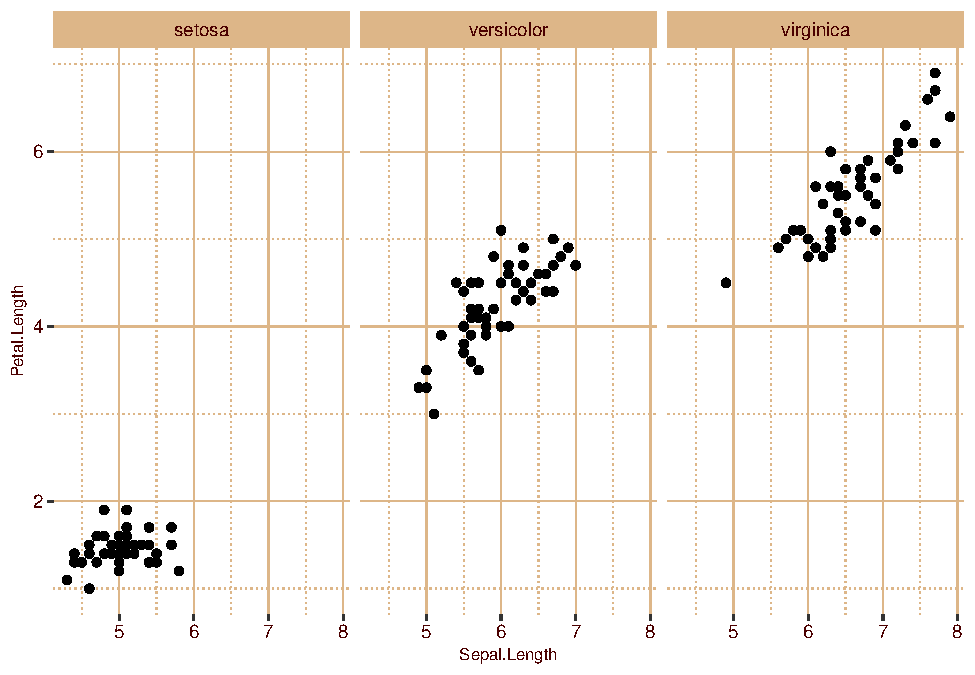
\includegraphics{R-markdown--world_airport_files/figure-latex/dotplotex-1.pdf}
\caption{\label{fig:dotplotex}Un exemple de graphique produit par R, inséré et légendé grâce à \emph{R Markdown}. S'il y a lieu, on précise la source des données, la cohorte et on explique comment lire le graphique.\\
\textbf{Source :} Jeu de données \texttt{iris}.\\
\textbf{Cohorte :} on peut insérer du code R dans la légende : il y a 150 points représentés dans ce graphique.\\
\textbf{Lecture :} Débrouillez-vous.}
\end{figure}

On peut insérer et légender des figures qui ne sont pas produites par R, comme illustré par la figure \ref{fig:logourca}.



\begin{Shaded}
\begin{Highlighting}[]
\NormalTok{knitr}\SpecialCharTok{::}\FunctionTok{include\_graphics}\NormalTok{(}\AttributeTok{path =} \StringTok{"logo\_URCA.pdf"}\NormalTok{)}
\end{Highlighting}
\end{Shaded}

\begin{figure}

{\centering 
\includegraphics[width=0.2\linewidth]{logo_URCA} 

}

\caption{Logo de l'Université de Reims Champagne-Ardenne.}\label{fig:logourca}
\end{figure}

On peut faire de même pour les tableaux, comme illustré par la Table \ref{tab:tableex} pour laquelle on a utilisé le package \textbf{kableExtra} \autocite{pkgkableExtra} pour modifier le style du tableau.



\begin{Shaded}
\begin{Highlighting}[]
\FunctionTok{library}\NormalTok{(}\StringTok{\textquotesingle{}knitr\textquotesingle{}}\NormalTok{)}
\FunctionTok{library}\NormalTok{(}\StringTok{\textquotesingle{}kableExtra\textquotesingle{}}\NormalTok{)}
\end{Highlighting}
\end{Shaded}

\begin{verbatim}
## Warning: package 'kableExtra' was built under R version
## 4.4.2
\end{verbatim}

\begin{Shaded}
\begin{Highlighting}[]
\CommentTok{\# set.seed(3)}
\CommentTok{\# un\_tableau \textless{}{-} table(sample(c("A", "B", "C"), 100, replace = TRUE), sample(1:4, 100, replace = TRUE))}
\CommentTok{\# kable(x = un\_tableau, format = \textquotesingle{}latex\textquotesingle{}, caption = "Un exemple de tableau accompagné de sa légende.", booktabs = TRUE) \%\textgreater{}\%}
\CommentTok{\#   kable\_styling(latex\_options = c(\textquotesingle{}striped\textquotesingle{})) \%\textgreater{}\%}
\CommentTok{\#   row\_spec(0, bold = TRUE)}
\FunctionTok{kable}\NormalTok{(}\AttributeTok{x =} \FunctionTok{head}\NormalTok{(iris,  }\AttributeTok{n =} \DecValTok{5}\DataTypeTok{L}\NormalTok{), }\AttributeTok{format =} \StringTok{"latex"}\NormalTok{,}
      \AttributeTok{caption =}  \StringTok{"Un exemple de tableau accompagné de sa légende."}\NormalTok{, }
      \AttributeTok{booktabs =} \ConstantTok{TRUE}\NormalTok{) }\SpecialCharTok{\%\textgreater{}\%}
  \FunctionTok{kable\_styling}\NormalTok{(}\AttributeTok{latex\_options =} \FunctionTok{c}\NormalTok{(}\StringTok{\textquotesingle{}striped\textquotesingle{}}\NormalTok{)) }\SpecialCharTok{\%\textgreater{}\%}
  \FunctionTok{row\_spec}\NormalTok{(}\DecValTok{0}\NormalTok{, }\AttributeTok{bold =} \ConstantTok{TRUE}\NormalTok{)}
\end{Highlighting}
\end{Shaded}

\begin{table}
\centering
\caption{\label{tab:tableex}Un exemple de tableau accompagné de sa légende.}
\centering
\begin{tabular}[t]{rrrrl}
\toprule
\textbf{Sepal.Length} & \textbf{Sepal.Width} & \textbf{Petal.Length} & \textbf{Petal.Width} & \textbf{Species}\\
\midrule
\cellcolor{gray!10}{5.1} & \cellcolor{gray!10}{3.5} & \cellcolor{gray!10}{1.4} & \cellcolor{gray!10}{0.2} & \cellcolor{gray!10}{setosa}\\
4.9 & 3.0 & 1.4 & 0.2 & setosa\\
\cellcolor{gray!10}{4.7} & \cellcolor{gray!10}{3.2} & \cellcolor{gray!10}{1.3} & \cellcolor{gray!10}{0.2} & \cellcolor{gray!10}{setosa}\\
4.6 & 3.1 & 1.5 & 0.2 & setosa\\
\cellcolor{gray!10}{5.0} & \cellcolor{gray!10}{3.6} & \cellcolor{gray!10}{1.4} & \cellcolor{gray!10}{0.2} & \cellcolor{gray!10}{setosa}\\
\bottomrule
\end{tabular}
\end{table}

D'autres packages sont dédiés à la mise en forme de tables pour leur incorporation dans un document \emph{R Markdown} ; citons notamment \textbf{gtsummary} \autocite{pkggtsummary}, \textbf{gt} \autocite{pkggt} et \textbf{flextable} \autocite{pkgflextable}. La table \ref{tab:exemplegtsum} présente un exemple de table mise en forme grâce à \textbf{gtsummary} puis incorporé au document final grâce à \textbf{kableExtra}. Consulter la documentation de ces packages pour de nombreux autres exemples.

\begin{verbatim}
## Warning: package 'gtsummary' was built under R version
## 4.4.2
\end{verbatim}

\begin{table}
\centering
\caption{\label{tab:exemplegtsum}Un exemple de table mise en forme grâce aux packages \textbf{gtsummary} et \textbf{kableExtra}.\\
\textbf{Source :} \emph{data.frame} \texttt{iris}.\\
\textbf{Lecture :} La longueur médiane des sépales des 50 iris de l'espèce \emph{setosa} est égale à 5.00. Entre parenthèses, sont indiqués les premier et troisième quartile (4.80, 5.20). La \emph{p-value} du test d'égalité des longueurs médianes entre les trois espèces d'iris est inférieure à 0.001.}
\centering
\begin{tabular}[t]{lccccc}
\toprule
\textbf{\textbf{Characteristic}} & \textbf{\textbf{N}} & \textbf{\makecell[c]{\textbf{setosa}\ \ \\N = 50}} & \textbf{\makecell[c]{\textbf{versicolor}\ \ \\N = 50}} & \textbf{\makecell[c]{\textbf{virginica}\ \ \\N = 50}} & \textbf{\textbf{p-value}}\\
\midrule
\cellcolor{gray!10}{Sepal.Length} & \cellcolor{gray!10}{150} & \cellcolor{gray!10}{5.00 (4.80, 5.20)} & \cellcolor{gray!10}{5.90 (5.60, 6.30)} & \cellcolor{gray!10}{6.50 (6.20, 6.90)} & \cellcolor{gray!10}{}\\
Sepal.Width & 150 & 3.40 (3.20, 3.70) & 2.80 (2.50, 3.00) & 3.00 (2.80, 3.20) & \\
\bottomrule
\multicolumn{6}{l}{\rule{0pt}{1em}\textsuperscript{1} Median (Q1, Q3)}\\
\end{tabular}
\end{table}





Les équations mathématiques centrées et numérotées peuvent également être référencées, comme l'équation \eqref{eq:equationex}.

\begin{equation}
 \mathbb{H}(p_1, \dots, p_n) := -\sum_{i=1}^n p_i \log p_i, \quad p_i \geq 0, i = 1, \dots, n \textrm{ and }  \sum_{i=1}^n p_i =1.
 \label{eq:equationex}
\end{equation}

De même, on peut faire référence aux théorèmes, propositions ou définitions que l'on déclare préalablement. Par exemple, le Théorème \ref{thm:theoex}. Consulter \textcite{xie_bookdown_2016} (partie 2.2.2) pour plus de détails.

\begin{theorem}[Théorème de Pythagore]
\protect\hypertarget{thm:theoex}{}\label{thm:theoex}Pour tout triangle rectangle, si on note \(c\) la longueur de l'hypothénuse et \(a\) et \(b\) les longueurs des deux autres côtés, alors
\[c^2 = a^2 + b^2.\]
\end{theorem}

\begin{proof}
Ceci est une preuve terminant par le symbole de fin de preuve.
\end{proof}

Pour citer un article, un ouvrage, une page web, etc, on remplit préalablement le fichier \texttt{biblio-cr-urca.bib} en déclarant les références dans la syntaxe de \emph{Bibtex} puis on insère la citation. Pour plus d'information sur le fonctionnement de \emph{R Markodown}, on pourra consulter \textcite{rmarkdown_refbook2018}. On peut également référencer des pages web en webographie ;
par exemple, on pourra consulter \textcite{canales_luna_top_2022} pour un état des lieux sur la popularité des logiciels en science des données.

\section*{Remerciements}\label{remerciements}
\addcontentsline{toc}{section}{Remerciements}

Merci la vie !

\appendix


\section{Annexes}\label{annexes}

On peut également ajouter une ou des partie(s) annexe(s) au document, permettant par exemple de détailler les procédures statistiques employées.

\textbf{urcadown} fournit également un ensemble d'utilitaires pour faciliter la création de thèmes graphiques homogènes. En guise d'illustration, on génère quelques palettes de couleurs à partir des couleurs définies par le bloc de code suivant et présentées dans la Table \ref{tab:couleurs}.

\begin{Shaded}
\begin{Highlighting}[]
\NormalTok{urcalightbrown }\OtherTok{\textless{}{-}} \StringTok{"\#D1AD55"}
\NormalTok{urcamediumbrown }\OtherTok{\textless{}{-}} \StringTok{"\#AE7433"}
\NormalTok{urcaheavybrown }\OtherTok{\textless{}{-}} \StringTok{"\#480000"}
\NormalTok{urcalightblue }\OtherTok{\textless{}{-}} \StringTok{"\#88C7FA"}
\NormalTok{urcamediumblue }\OtherTok{\textless{}{-}} \StringTok{"\#1A9DDD"}
\NormalTok{urcaheavyblue }\OtherTok{\textless{}{-}} \StringTok{"\#365A8E"}
\NormalTok{senolive }\OtherTok{\textless{}{-}} \StringTok{"\#76bc21"}
\NormalTok{sendarkgreen }\OtherTok{\textless{}{-}} \StringTok{"\#007934"}
\NormalTok{senlightgreen }\OtherTok{\textless{}{-}} \StringTok{"\#00ae42"}
\NormalTok{darkpink }\OtherTok{\textless{}{-}} \StringTok{"\#DB6761"}
\NormalTok{clay }\OtherTok{\textless{}{-}} \StringTok{"\#D95F02"}
\NormalTok{sand }\OtherTok{\textless{}{-}} \StringTok{"\#FED976"}
\NormalTok{shadedpurple }\OtherTok{\textless{}{-}} \StringTok{"\#CD7FC5"}
\end{Highlighting}
\end{Shaded}

\begin{verbatim}
## Loading required package: rmarkdown
\end{verbatim}

\begin{verbatim}
## Warning: package 'rmarkdown' was built under R version
## 4.4.2
\end{verbatim}

\begin{verbatim}
## Loading required package: bookdown
\end{verbatim}

\begin{verbatim}
## Warning: package 'bookdown' was built under R version 4.4.2
\end{verbatim}

\begin{verbatim}
## Loading required package: formatR
\end{verbatim}

\begin{verbatim}
## Warning: package 'formatR' was built under R version 4.4.2
\end{verbatim}

\begin{verbatim}
## Loading required package: magrittr
\end{verbatim}

\begin{verbatim}
## Loading required package: tidyverse
\end{verbatim}

\begin{verbatim}
## Warning: package 'tidyverse' was built under R version
## 4.4.2
\end{verbatim}

\begin{verbatim}
## Warning: package 'tidyr' was built under R version 4.4.2
\end{verbatim}

\begin{verbatim}
## Warning: package 'lubridate' was built under R version
## 4.4.2
\end{verbatim}

\begin{verbatim}
## -- Attaching core tidyverse packages ---- tidyverse 2.0.0 --
## v forcats   1.0.0     v stringr   1.5.1
## v lubridate 1.9.3     v tibble    3.2.1
## v purrr     1.0.2     v tidyr     1.3.1
## v readr     2.1.5
\end{verbatim}

\begin{verbatim}
## -- Conflicts ---------------------- tidyverse_conflicts() --
## x tidyr::extract()    masks magrittr::extract()
## x dplyr::filter()     masks stats::filter()
## x dplyr::group_rows() masks kableExtra::group_rows()
## x dplyr::lag()        masks stats::lag()
## x purrr::set_names()  masks magrittr::set_names()
## i Use the conflicted package (<http://conflicted.r-lib.org/>) to force all conflicts to become errors
\end{verbatim}

\begin{table}

\caption{\label{tab:couleurs}Un exemple de table mise en forme grâce aux packages \textbf{gtsummary} et \textbf{kableExtra}.\\
\textbf{Source :} \emph{data.frame} \texttt{iris}.\\
\textbf{Lecture :} La longueur médiane des sépales des 50 iris de l'espèce \emph{setosa} est égale à 5.00. Entre parenthèses, sont indiqués les premier et troisième quartile (4.80, 5.20). La \emph{p-value} du test d'égalité des longueurs médianes entre les trois espèces d'iris est inférieure à 0.001.}
\centering
\begin{tabular}[t]{l|l|l}
\hline
\textbf{Nom couleur} & \textbf{Code hexa} & \textbf{Code RGB}\\
\hline
\cellcolor[HTML]{D1AD55}{urcalightbrown} & \cellcolor[HTML]{D1AD55}{\#D1AD55} & \cellcolor[HTML]{D1AD55}{209, 173, 85}\\
\hline
\cellcolor[HTML]{AE7433}{urcamediumbrown} & \cellcolor[HTML]{AE7433}{\#AE7433} & \cellcolor[HTML]{AE7433}{174, 116, 51}\\
\hline
\cellcolor[HTML]{480000}{urcaheavybrown} & \cellcolor[HTML]{480000}{\#480000} & \cellcolor[HTML]{480000}{72, 0, 0}\\
\hline
\cellcolor[HTML]{88C7FA}{urcalightblue} & \cellcolor[HTML]{88C7FA}{\#88C7FA} & \cellcolor[HTML]{88C7FA}{136, 199, 250}\\
\hline
\cellcolor[HTML]{1A9DDD}{urcamediumblue} & \cellcolor[HTML]{1A9DDD}{\#1A9DDD} & \cellcolor[HTML]{1A9DDD}{26, 157, 221}\\
\hline
\cellcolor[HTML]{365A8E}{urcaheavyblue} & \cellcolor[HTML]{365A8E}{\#365A8E} & \cellcolor[HTML]{365A8E}{54, 90, 142}\\
\hline
\cellcolor[HTML]{76bc21}{senolive} & \cellcolor[HTML]{76bc21}{\#76bc21} & \cellcolor[HTML]{76bc21}{118, 188, 33}\\
\hline
\cellcolor[HTML]{007934}{sendarkgreen} & \cellcolor[HTML]{007934}{\#007934} & \cellcolor[HTML]{007934}{0, 121, 52}\\
\hline
\cellcolor[HTML]{00ae42}{senlightgreen} & \cellcolor[HTML]{00ae42}{\#00ae42} & \cellcolor[HTML]{00ae42}{0, 174, 66}\\
\hline
\cellcolor[HTML]{DB6761}{darkpink} & \cellcolor[HTML]{DB6761}{\#DB6761} & \cellcolor[HTML]{DB6761}{219, 103, 97}\\
\hline
\cellcolor[HTML]{D95F02}{clay} & \cellcolor[HTML]{D95F02}{\#D95F02} & \cellcolor[HTML]{D95F02}{217, 95, 2}\\
\hline
\cellcolor[HTML]{FED976}{sand} & \cellcolor[HTML]{FED976}{\#FED976} & \cellcolor[HTML]{FED976}{254, 217, 118}\\
\hline
\cellcolor[HTML]{CD7FC5}{shadedpurple} & \cellcolor[HTML]{CD7FC5}{\#CD7FC5} & \cellcolor[HTML]{CD7FC5}{205, 127, 197}\\
\hline
\end{tabular}
\end{table}

Un exemple de table mise en forme grâce aux packages \textbf{gtsummary} et \textbf{kableExtra}.\\
\textbf{Source :} \emph{data.frame} \texttt{iris}.\\
\textbf{Lecture :} La longueur médiane des sépales des 50 iris de l'espèce \emph{setosa} est égale à 5.00. Entre parenthèses, sont indiqués les premier et troisième quartile (4.80, 5.20). La \emph{p-value} du test d'égalité des longueurs médianes entre les trois espèces d'iris est inférieure à 0.001. Exemples de couleurs compatibles avec la charte graphique de l'URCA, accompagnées de leurs codes hexadécimaux et RGB.



\pagebreak
\addcontentsline{toc}{section}{Bibliographie}
\printbibliography[title={Bibliographie}, nottype=online, nottype=manual]
\printbibliography[title={Webographie}, type=online]
\printbibliography[title={Packages référencés}, type=manual]


\end{document}
